\subsection{Reversi}

\begin{figure}
	\centering
	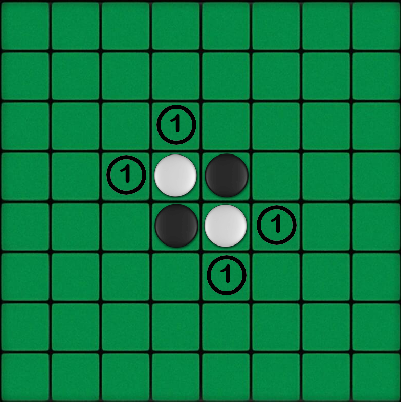
\includegraphics[width=0.5\textwidth]{pics/reversi_start.png}	
	\caption{Reversi Startaufstellung der Spielsteine. Mit 1 sind die m\"{o}glichen Z\"{u}ge des schwarzen Spielers angegeben. Screenshot von: \cite{PlayReversi}.}
	\label{fig:reversi_start}
\end{figure}

In diesem Abschnitt werden die grundlegenden Spielregeln\footnote{$https://de.wikipedia.org/wiki/Othello_(Spiel)$} von Reversi, so wie sie ebenfalls im vorliegenden Projekt Anwendung finden, vorgestellt.

Reversi ist ein kompetitives Spiel, bei dem die Teilnehmer in einer vorgegebenen Reihenfolge Z\"{u}ge machen d\"{u}rfen. Bei zwei Spielern bedeutet das, dass sich diese abwechseln, bei mehr als zwei geht es reihum. 

\"{U}blicherweise ist das Spielfeld, wie in Abbildung \ref{fig:reversi_start} dargestellt, ein Quadrat der Gr\"{o}\ss e 8x8, wobei Abwandlungen in andere Dimensionen grunds\"{a}tzlich m\"{o}glich sind. Ein typischer Startzustand zeigt sich darin, dass bereits zwei Steine der beiden Spieler, also ingesamt vier, in der Mitte des Feldes in Form einer 2x2 Anordnung platziert sind. Die Steine der jeweiligen Teilnehmer sind dabei diagonal angeordnet.

Jeder Spieler hat eine Farbe beziehungsweise ein Symbol f\"{u}r seine gelegten Steine. Ein Zug besteht darin, den eigenen Spielstein angrenzend an einen gegnerischen Stein so auf dem Spielfeld zu platzieren, sodass mindestens ein gegnerischer Spielstein eingeschlossen wird.  Sobald der eigene Spielstein positioniert ist, werden alle gegnerischen, die zwischen dem neuen und bereits vorhandenen Steinen liegen, so umgekehrt, dass sie die Farbe oder das Symbol des derzeitigen Spielers annehmen. Ist kein eigener Spielzug m\"{o}glich, kann also kein gegnerischer Stein durch einen eigenen ersetzt werden, muss der Spieler diesen Spielzug aussetzen. 

Ziel ist es, m\"{o}glichst viele Steine der eigenen Farbe oder mit dem eigenen Symbol auf dem Feld zu haben. Das Spiel ist beendet, sobald beide Spieler direkt hintereinander passen beziehungsweise beide keine Z\"{u}ge mehr machen k\"{o}nnen. Gewonnen hat entsprechend derjenige, der mehr Spielsteine auf dem Feld liegen hat. Falls beide Teilnehmer die gleiche Anzahl haben, so ist der Spielausgang unentschieden.

\subsection{ReversiXT}
Um das Spiel etwas interessanter und f\"{u}r unsere KI etwas herausfordernder zu gestalten, lassen wir derzeit Spielfeldgr\"{o}\ss en bis zu 15x15 Feldern zu, die Startposition der Anfangssteine darf hierbei beliebig sein und muss nicht mittig angelegt werden. Gr\"{o}\ss ere Spielgr\"{o}\ss en k\"{o}nnen in der Klasse AlphaGoZeroConstants in der Konstante \glqq DIMENSION\_PLAYGROUND\grqq{} gesetzt werden, der hierf\"{u}r ben\"{o}tigte Wert ist das Maximum aus der Spielfeldh\"{o}he und der -breite. Bei einer \"{A}nderung muss jedoch das Modell von Grund auf neu trainiert werden.\\
Zudem lassen wir sogenannte L\"{o}cher im Spielfeld zu, also Felder auf die keiner der Spieler ziehen kann. Das Setzen auf anliegende Felder ist somit sicherer als mittig im Spielfeld, da die Spielsteine nicht vom Feld des Loches aus umgekehrt werden k\"{o}nnen.